\documentclass{article}
\usepackage{graphicx}
\usepackage{caption}
\usepackage{float}

\begin{document}
\section{Maillage}

Avant de générer le maillage, il est nécessaire d'étudier la géométrie de l'aimant. On remarque que les côtés  \textit{\( \Gamma_{Channel} \)} sont arrondis, avec des longueurs \textit{\( \Gamma_{in}\)} et \textit{\( \Gamma_{out}\)} de 100 mm, et un angle de \( \frac{\pi}{18} \) entre ces deux rayons.

Pour tracer \textit{\( \Gamma_{Channel} \)}, nous partons des deux points \((0,0)\) et \((0, r_i)\), où \( r_i \) représente la largeur de l'aimant. En utilisant l'angle donné, nous pouvons calculer la position du centre du cercle passant par ces deux points. Nous reproduisons ensuite cette construction à une hauteur de 100 mm en ajoutant cette valeur aux coordonnées du centre du cercle.

L’arc de cercle satisfait la relation trigonométrique suivante :
\begin{equation}
\sin\left(\frac{\theta}{2}\right) = \frac{d}{2R}
\end{equation}
Avec :
\begin{equation}
\sin\left(\frac{\pi}{36}\right) = \frac{r_i}{2R}
\end{equation}
Nous en déduisons :
\begin{equation}
R = \frac{r_i}{2 \sin(\pi/36)}
\end{equation}

Grâce à cette relation, nous obtenons la base du maillage :

\begin{figure}[H]
    \centering
    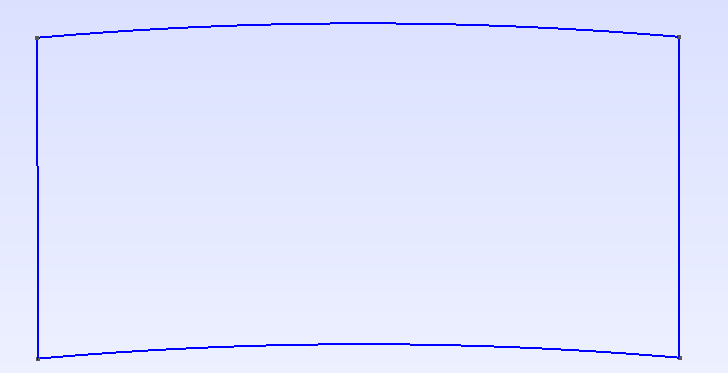
\includegraphics[width=0.7\textwidth]{images/gmsh_1.png}
    \caption{Base du maillage}
\end{figure}

Ensuite, nous ajoutons le cercle central \textit{\( \Gamma_{cool_1} \) }, dont le centre est situé en \( (r_i/2, l/2) \) et de rayon \( r_1/2 \). Enfin, nous insérons les fentes \textit{\( \Gamma_{cool_2} \) }. Ne disposant pas d’informations précises sur leur position exacte, nous avons choisi de les placer arbitrairement. Leur base est définie par les points \((10,8)\) et \((10,88)\). À partir des données disponibles, nous générons les autres points en respectant une largeur \( w_2 = 1.1 \) mm et une longueur de 5.9 mm. 

Le maillage obtenu est le suivant :

\begin{figure}[H]
    \centering
    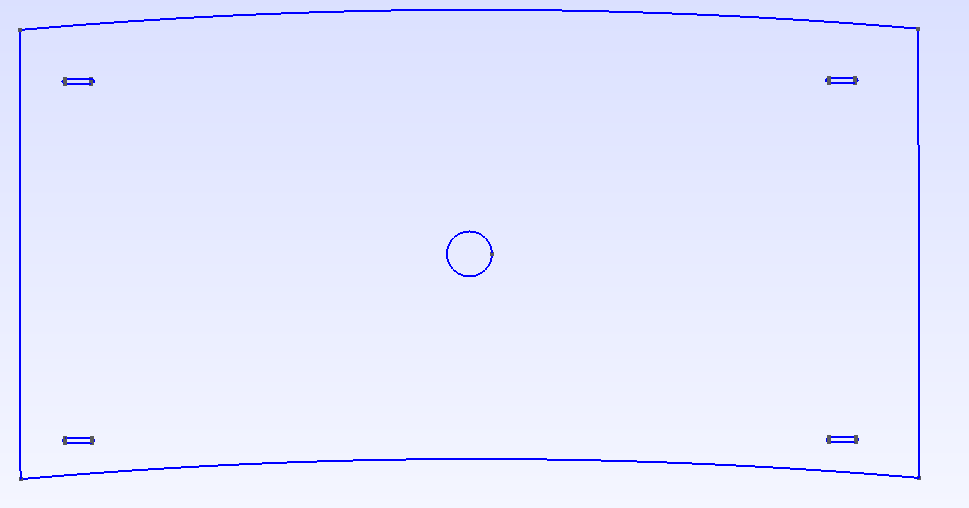
\includegraphics[width=0.7\textwidth]{images/gmsh_2.png}
    \caption{Maillage généré avec les fentes}
\end{figure}

Une fois cette base obtenue, nous procédons à son extrusion de 4 mm, comme demandé, avant d'appliquer le maillage final.

\begin{figure}[H]
    \centering
    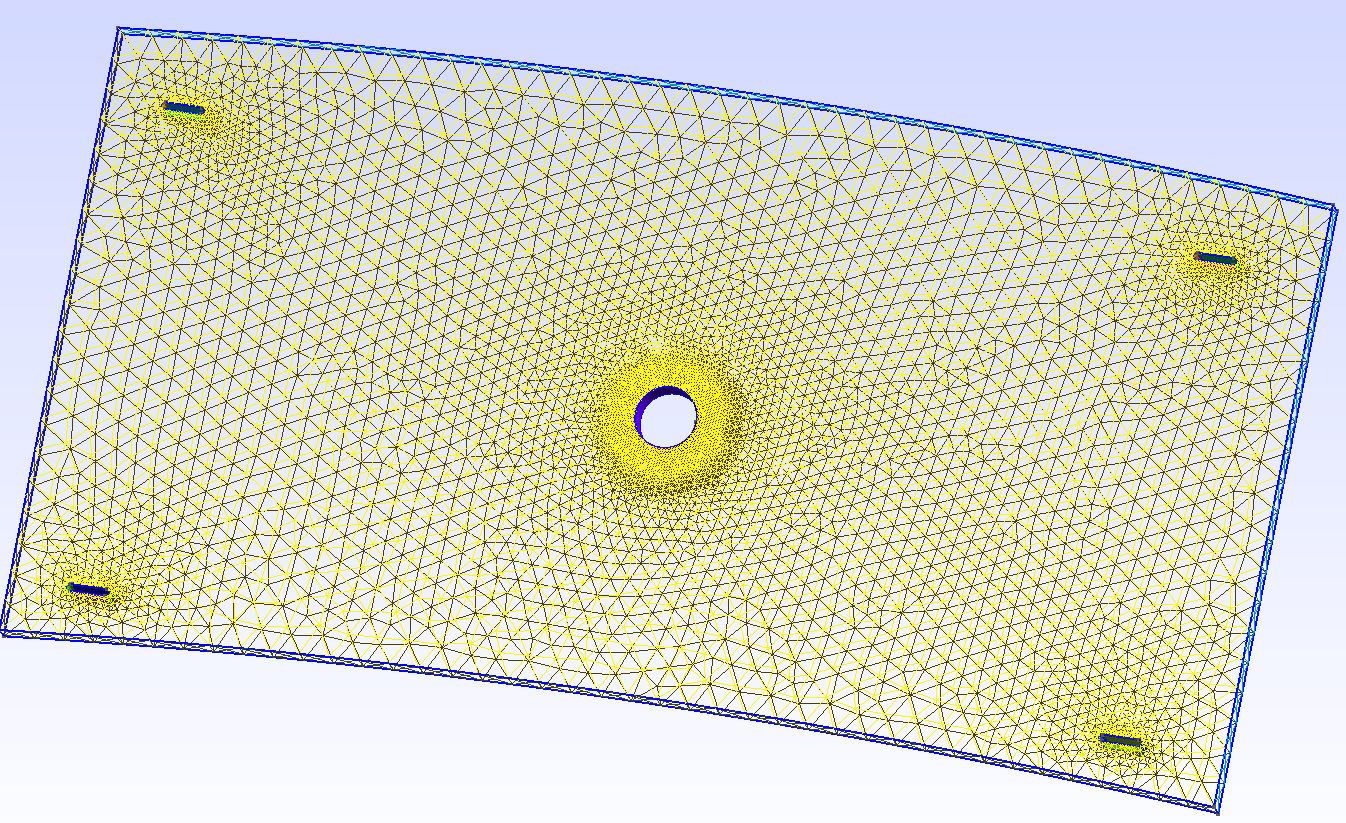
\includegraphics[width=0.7\textwidth]{images/gmsh_3.png}
    \caption{Maillage final après extrusion}
\end{figure}

Le maillage est raffiné au niveau des zones arrondies afin d'améliorer leur approximation et garantir une meilleure précision.

\section{Visualisation}

La visualisation a été faite à partir du fichier fourni 

\subsection{Topologie du maillage}

Pour extraire les parties du maillage voulu nous avons utilisé des clip en activant l'option 'crinkle clip', 
cela permet de visualiser les partie du maillage raffiné ou grossière de près.

\begin{figure}[H]
    \centering
    \includegraphics[width=0.7\textwidth]{images/maillage_raffiné.png}
    \caption{Maillage raffiné}
\end{figure}

Sur le maillage raffiné, on distingue les petites mailles. 
La partie du maillage raffiné se situe près des trous, 
ce qui permet une meilleure approximation de la forme que l'on souhaite représenter.

\begin{figure}[H]
    \centering
    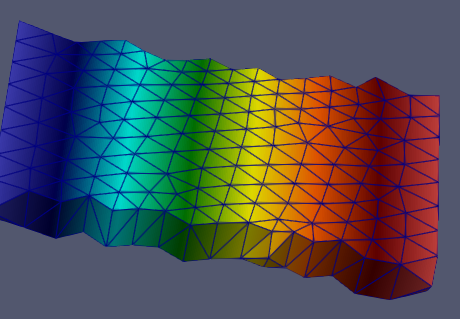
\includegraphics[width=0.7\textwidth]{images/maillage_grossier.png}
    \caption{Maillage grossier}
\end{figure}

Sur le maillage grossier, on observe que les mailles ont la largeur de notre aimant. 
Elles ne sont pas coupées, car nous avons choisi de les conserver entières dans notre coupe. 
Ce maillage grossier se trouve loin des trous et des formes arrondies, 
ce qui permet de réduire le temps de calcul et l’espace de stockage tout en conservant les détails essentiels.

\subsection{Visualisation du champs éléctrique en fonction de la chaleur}
Pour visualiser le champs éléctrique en fonction de la chaleur 
nous avons affiché les 'streamlines' sur le champs éléctrique que l'on a seed en utilisant une sphere au centre de notre aimant. 
Pour permettre de visualiser l'effet de la chaleur la coloration de ces 'streamlines' est en fonction de la chaleur.
\begin{figure}[h]
    \centering
    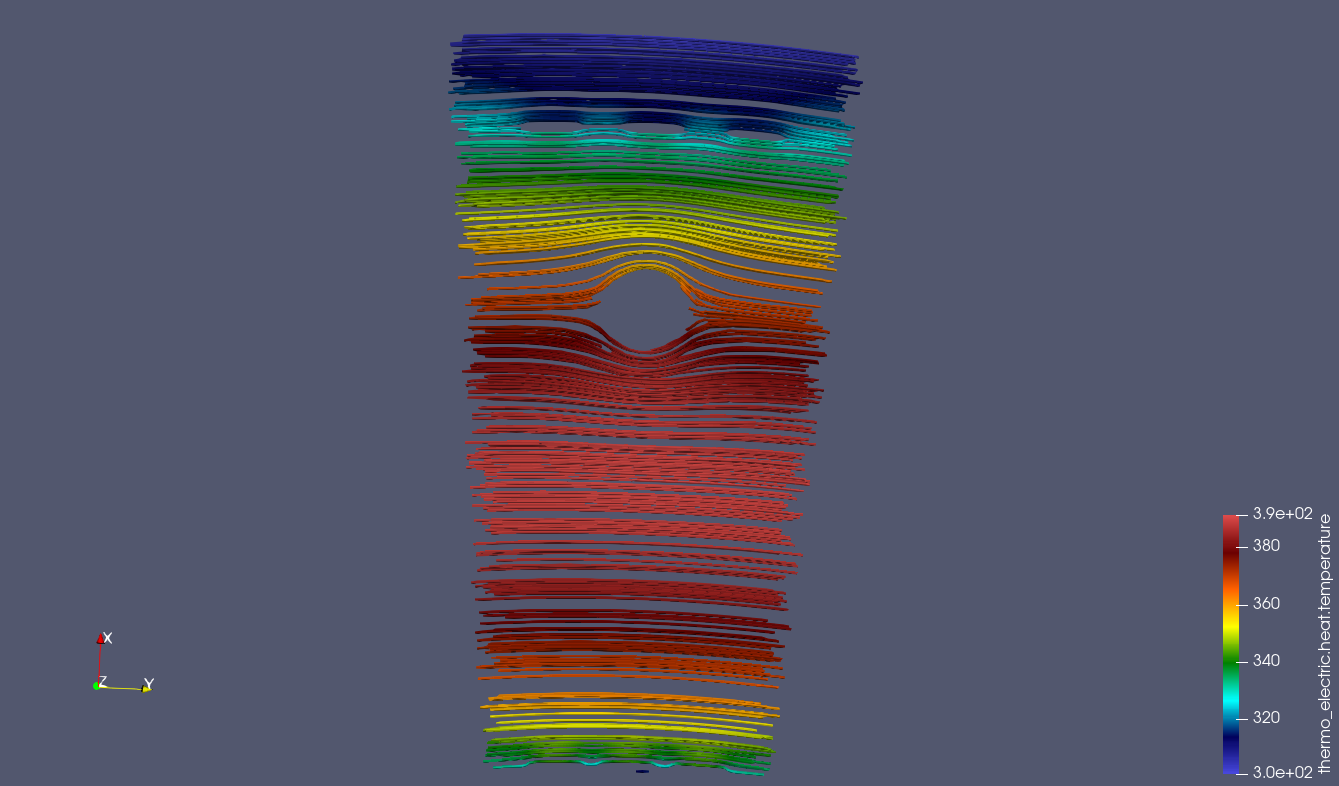
\includegraphics[width=0.7\textwidth]{images/champ_electrique.png}
    \caption{Champs éléctrique en fonction de la chaleur}
\end{figure}
\subsection{Extraction d'isosurface en fonction du potentiel éléctrique}
Pour extraire les isosurface correspondant au valuer 390, 390.5 et 391 on selectionne le filtre 'contour' sur lequel on ajoute les valeurs voulu.
Pour faire apparaitre le potentiel éléctrique on choisi la couleur de celui ci. 
\begin{figure}[h]
    \centering
    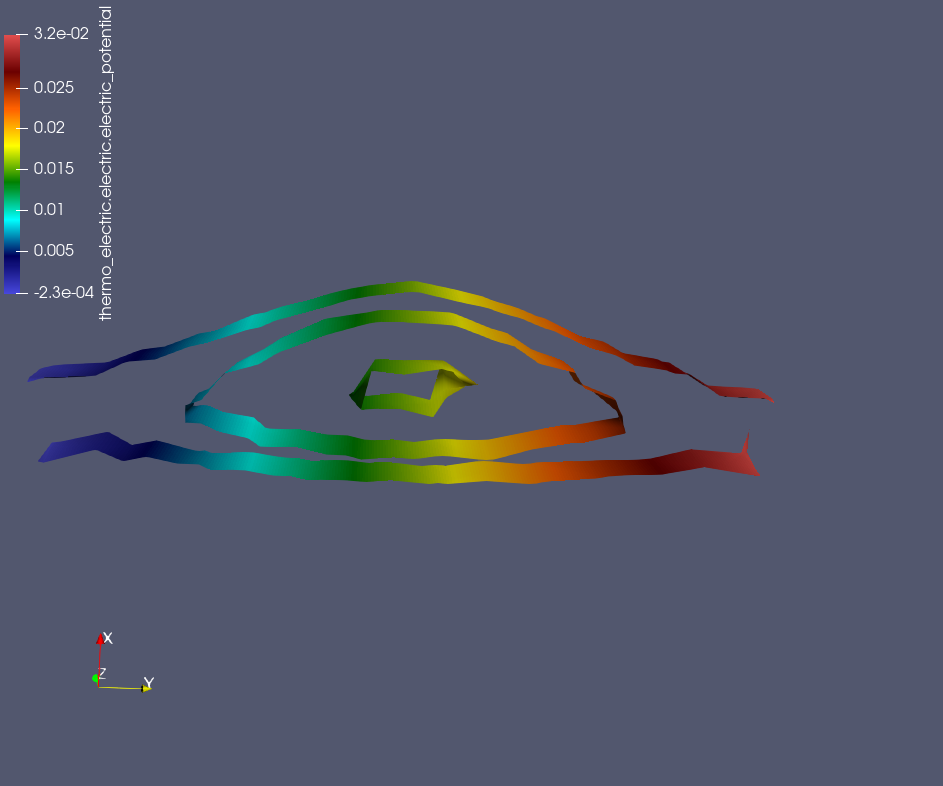
\includegraphics[width=0.7\textwidth]{images/isosurface.png}
    \caption{Isosurface correspondant au valeur 390, 390.5 et 391 en fonction du potentiel éléctrique}
\end{figure}
\end{document} 